\documentclass{swfcthesis}

\addbibresource{thesis.bib}    % 参照教程自己去写一个.bib文件

\begin{document}

\Title{论文标题}
\Author{作者姓名}
\Advisor{指导教师姓名}
\AdvisorTitle{指导教师职称}
\AdvisorInfo{指导教师简介(约百余字)}
\Month{六}
\Year{二〇一七}
\Subject{计算机科学与技术专业}    %专业名称(比如 电子信息工程专业)
\Abstract{这里写论文摘要(约两百字)}
\Keywords{这里写关键字,比如 电阻, 电容}
\Acknowledgments{这里写鸣谢(约百余字)}
\enTitle{英文标题}
\enAuthor{英文姓名}
\enAbstract{英文摘要}
\enKeywords{英文关键字}

%%% 下面六行不要动!
\makepreliminarypages% 封面
\frontmatter          
\tableofcontents     % 目录
\listoffigures       % 插图目录
\listoftables        % 表格目录
\mainmatter

\chapter{第一章标题}


正文部分从此开始。可以参考模版目录中的各章节tex文件来写。

\section{图片与表格}

如果需要插入图片与表格的话,可以参考下面的简单例子。

\subsection{图片示例}

下面是插入图片的示例:

\begin{figure}[!ht]
  \centering
  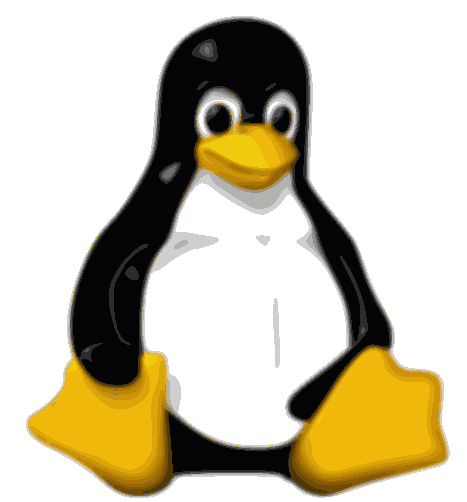
\includegraphics[width=.5\textwidth]{tux}
  \caption{图片示例}
  \label{fig:hello}
\end{figure}

\subsection{表格示例}

下面是一个表格的例子:

\begin{table}[!ht]
  \centering
  \begin{tabular}{|r|c|l|}
    \hline
    Hello&world&Hello, world!\\hline
    Hello&world&Hello, world!\\hline
  \end{tabular}
  \caption{表格示例}
  \label{tab:hello}
\end{table}

\chapter{又一章标题}

接着写吧接着写吧接着写吧接着写吧

%%% 正文部分到此结束。下面是『参考文献』、『指导教师简介』、『鸣谢』、『附录』

%% 不要动下面四行!
\Appendix{}
\printbibliography[heading={bibintoc},title={参考文献}] % 输出参考文献
\advisorinfopage{}                 % 输出指导教师简介
\acknowledgmentspage{}             % 输出鸣谢

%%% 下面是附录部分,可以没有。

\chapter{我也不知道为什么要写附录} %附录一

可以参考模版目录中的 appendix.tex 文件来写。

\chapter{主要程序代码} %附录二

% 插入程序代码
\inputminted[fontsize=\small]{c}{figs/hello.c}

% 也可以这样
\begin{listing}[H]
  \inputminted{c}{figs/hello.c}
  \caption{Hello, world!}
  \label{lst:hello}
\end{listing}  

\end{document} % 结束。不要动下面几行!

%%% Local Variables:
%%% mode: latex
%%% TeX-master: t
%%% End:
